\documentclass{MScthesisITEM}

% this package is just to generate text for demo-purposes
\usepackage{blindtext}


\title{Detecting DNS tunneling using machine learning} % The title of your assignement; NB use \newlinetitle to start a newline
\author{Terje Kristoffer Skow} % Your firstname and lastname
\professor{Than Van Do, ITEM} % Affiliation = ITEM for instance
\supervisor{Hai Ngyuen, Telenor Research}

%% Uncomment the following in case you want subfigures; note that there will be a warning for the caption package
% \let\subcaption\undefined
% \let\subfloat\undefined
% \usepackage[bf]{caption}
% \usepackage{subcaption}

\DeclareGraphicsExtensions{.pdf,.jpg}
\graphicspath{{./figs/}}

\loadglsentries{glossary}
\makeglossaries

\begin{document}
\selectlanguage{english}
\pagenumbering{roman}
\pagestyle{plain}

%% Only for the project; comment out the line below for the master's thesis; the front page will be generated automatically by DAIM
\titleITEM

%% Only for the master's thesis; for the project report the description is taken from It's Learning and added by the department
% \selectlanguage{english} % Change to 'norsk' if you are writing in Norwegian
% \begin{titlingpage}

\noindent
\begin{tabular}{@{}p{4cm}l}
\textbf{Title:} 	& \thetitle \\
\textbf{Student:}	& \theauthor \\
\end{tabular}

\vspace{4ex}
\noindent\textbf{Problem description:}
\vspace{2ex}

\noindent \Blindtext[2][1]
\vspace{6ex}

\noindent
\begin{tabular}{@{}p{4cm}l}
\textbf{Responsible professor:} 	& \theprofessor \\
\textbf{Supervisor:}			& \thesupervisor \\
\end{tabular}

\end{titlingpage}
% \cleardoublepage

%% There must be an abstract in English, even though the main text is in Norwegian
\selectlanguage{english}
\pagestyle{empty}
\begin{abstract}
\end{abstract}
\cleardoublepage

%% Only for the master's thesis; if the main text is in English and you can write Norwegian, there must be an abstract in Norwegian as well.
% \selectlanguage{norsk}
% \pagestyle{empty}
\renewcommand{\abstractname}{Sammendrag}
\begin{abstract}
\noindent Sikkerheten til nesten all offentlig nøkkel-kryptografi er basert på et vanskelig beregnbarhetsproblem. Mest velkjent er problemene med å faktorisere heltall i sine primtallsfaktorer, og å beregne diskrete logaritmer i endelige sykliske grupper. I de to siste tiårene, har det imidlertid dukket opp en rekke andre offentlig nøkkel-systemer, som baserer sin sikkerhet på helt andre type problemer. Et lovende forslag, er å basere sikkerheten på vanskeligheten av å løse store likningsett av flervariable polynomlikninger. En stor utfordring ved å designe slike offentlig nøkkel-systemer, er å integrere en effektiv ``falluke'' (trapdoor) inn i likningssettet. En ny tilnærming til dette problemet ble nylig foreslått av Gligoroski m.f., hvor de benytter konseptet om kvasigruppe-strengtransformasjoner (quasigroup string transformations). I denne masteroppgaven beskriver vi en metodikk for å identifisere sterke og svake nøkler i det nylig foreslåtte multivariable offentlig nøkkel-signatursystemet MQQ-SIG, som er basert på denne idéen.

Vi har gjennomført et stort antall eksperimenter, basert på Gröbner basis angrep, for å klassifisere de ulike parametrene som bestemmer nøklene i MQQ-SIG. Våre funn viser at det er store forskjeller i viktigheten av disse parametrene. Metodikken består i en klassifisering av de forskjellige parametrene i systemet, i tillegg til en innføring av konkrete kriterier for hvilke nøkler som bør velges. Videre, har vi identifisert et unødvendig krav i den originale spesifikasjonen, som krevde at kvasigruppene måtte oppfylle et bestemt kriterie. Ved å fjerne denne betingelsen, kan nøkkel-genererings-algoritmen potensielt øke ytelsen med en stor faktor. Basert på alt dette, foreslår vi en ny og forbedret nøkkel-genereringsalgoritme for MQQ-SIG, som vil generere sterkere nøkler og være mer effektiv enn den originale nøkkel-genereringsalgoritmen.  
\end{abstract}
% \cleardoublepage

\selectlanguage{english}% Change to 'norsk' if you are writing in Norwegian

\renewcommand{\abstractname}{Preface}
\begin{abstract}
\noindent \blindtext 
\end{abstract}
\cleardoublepage

% similarly you may add a separate acknowledgments page

\tableofcontents*
\cleardoublepage

%% include if relevant
\listoffigures
\cleardoublepage

%% include if relevant
\listoftables
\cleardoublepage

%% include if relevant
\listofalgorithms
\addcontentsline{toc}{chapter}{List of Algorithms}
\cleardoublepage


%% include if relevant
\printglossary[title=List of Acronyms,type=\acronymtype] % prints just the list of acronyms
\cleardoublepage

\pagenumbering{arabic}
\pagestyle{ruled}
%\chapter{Example}
\label{chp:example} 

Here is an example of how to use acronyms such as \gls{ntnu}. The second time only \gls{ntnu} is shown and if there were several you would write \glspl{ntnu}. And here is an example\footnote{A footnote} of citation~\cite{Author:year:XYZ}. 

\Blindtext[3][1]

\begin{figure}
\centering
% dummy figure replacement 
\begin{tabular}{@{}c@{}}
\rule{.5\textwidth}{.5\textwidth} \\
\end{tabular}
\caption{\label{fig:example}A figure}
\end{figure}

\section{First section}\label{sec:first_section}

\subsection{First subsection with some \texorpdfstring{$\mathcal{M}ath$}{Math} symbol}\label{sec:first_ssection}

\blindtext
\begin{itemize}[topsep=-1em,parsep=0em,itemsep=0em] % see http://mirror.ctan.org/macros/latex/contrib/enumitem/enumitem.pdf for details about the parameters
 \item item1
 \item item2
 \item ...
\end{itemize}

\subsection{Mathematics}

\blindmathtrue
\blindtext

\begin{proposition}\label{def:a_proposition}
A proposition... (similar environments include: theorem, corrolary, conjecture, lemma)

\end{proposition}

\begin{proof}
\vspace*{-1em} % Adjust the space when parskip is set to 1em
And its proof.
\end{proof}

\begin{table}
\caption{\label{tab:example}A table}
\centering
\begin{tabular}[b]{| c | c | c | c | c |}
\hline
a & b & c & d & e \\ \hline
f & g & h & i & j \\ \hline
k & l & m & n & o \\ \hline
p & q & r & s & t \\ \hline
u & v & w & x & y \\ \hline
z & æ & ø & å &   \\ \hline
\end{tabular} 
\end{table}

\subsection{Source code example}

% \floatname{algorithm}{Source code} % if you want to rename 'Algorithm' to 'Source code'
\begin{algorithm}[h]
  \caption{The Hello World! program in Java.}
  \label{hello_world}
  % alternatively you may use algorithmic, or lstlisting from the listings package
  \begin{verbatim}
  
class HelloWorldApp {
  public static void main(String[] args) {
    //Display the string
    System.out.println("Hello World!");
  }
}
\end{verbatim}
\end{algorithm}

You can refer to figures using the predefined command like \fref{fig:example}, to pages like \pref{fig:example}, to tables like \tref{tab:example}, to chapters like \Cref{chp:example} and to sections like \Sref{sec:first_section} and you may define similar commands to refer to proposition, algorithms etc.

%% include here the other chapters
\chapter{DNS}
\label{chp:dns}

\section{Introduction}

\gls{dns} is an important part for the internet. It is a system of distributed databases which contains the information about all the domains. In the mid and late 1980s did the previous system \texttt{HOST.TXT} encounter problems \cite{Mockapetris:1988:DDN:52324.52338} which lead to the creation and standardisation of the so-called \gls{dns}. Since that has the \Gls{dns} system been updated and configured many times. It needed to be able to maintain a fast response time as the database grew larger. This was solved by using a hierarchical set up. This means that each server only has a limited information and sends the request to a new server until it reaches the correct server. It started with one root server, which has expanded to 13 today. Each layer of the hierarchy is called a zone, and it delegates the responsibility for underlying zones delimited by the \texttt{dot} in the request name. This is illustrated in \fref{fig:namespace}.

\begin{figure}
\centering
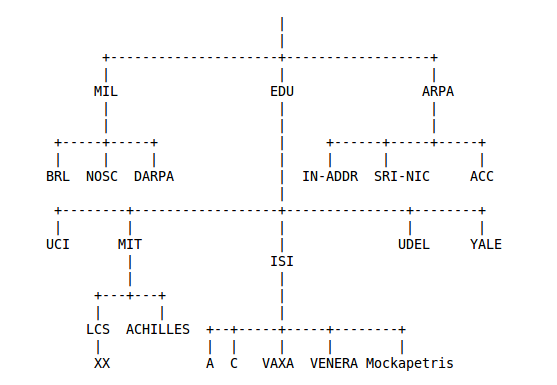
\includegraphics[scale=0.5]{figs/namespace_example.png}
\caption{\label{fig:namespace}Example of name spaces of a root with MIL, EDU and ARPA as immediate subdomains. Each leaf is a domain \citep{mockapetris1987domain}.}
\end{figure}



\section{Structure}
The data in the databases are called \gls{rr} and contains the information about what the server do with the request. It has the following fields \cite{mockapetris1983domain}:
\begin{itemize} 
\item NAME -- the owner name of the record.
\item TYPE -- what type of record this is, name-to-IP (A) or IP-to-name (PTR).
\item CLASS -- define the class of the record, usually \texttt{IN} for internet. It is not widely use and not important for this paper.
\item TTL -- an integer which says how long the record should be cached by the server receiving the response.
\item RDLENGTH -- Specifies the length of the payload in number of octets. One octet is one octet of bits which corresponds to one character
\item RDATA -- the payload of the record. The format and length varies depending on the TYPE and CLASS of the \Gls{rr}.
\end{itemize}

\gls{dns} was first implemented with around 15 different \gls{rr} TYPE, which has now increased to over 30 \cite{farnham2013detecting} as a result of the development of the internet. The most notable values for TYPE are:

\begin{itemize}
\item A -- the payload will contain the ipv4 address of the hostname requested. This is the most used TYPE
\item AAAA -- contains the ipv6 address of the hostname.
\item CNAME -- canonical name, respond with the correct alias of the hostname.
\item MX -- the mail exchange for the domain
\item TXT -- a text response with large payload, can be used in many ways and are an important type in \gls{dns} tunneling.
\item PTR -- pointer record. Used to map a hostname to an IP-address, commonly known as a reverse lookup.
\item NS -- authoritative name server for the domain
\end{itemize}

The 'A' type \gls{rr} for telenor.no at the name server will look something like this:

\begin{table}
\centering
\begin{tabular}[c]{|l|l|}
\hline
\textbf{Field} & \textbf{Value} \\ \hline
NAME & telenor.no \\ \hline
TYPE & A \\ \hline
CLASS & IN \\ \hline
TTL & 300 \\ \hline
RDLENGTH & 15 \\ \hline
RDATA & 153.110.156.145 \\ \hline

\end{tabular}
\caption{\label{tab:rrexample}Example of \gls{rr} for telenor.no}
\end{table}


\section{How it works}
To explain of \Gls{dns} works is an example the easiest way

When a request goes through \Gls{dns} it starts in the root zone, where it sent down the hierarchy to the \texttt{.no} zone.



Normally a \Gls{dns} server in an enterprise does not send requests directly to the internet, but use an internal \Gls{dns} server instead. If you are the owner of the authoritative server for a domain, you can control the responses. This is what a \Gls{dns} tunnel exploits, which will be explained in more details in the next section. 





 
\chapter{DNS Tunneling}
\label{chp:dns_tunneling}



\Gls{dns} tunneling was first used by people who exploited that \Gls{dns} was not monitored in network you had to pay to use, e.g. hotels and cafés. It was used as an \Gls{vpn} tunnel. In later years it has been discovered that in enterprises the \Gls{dns} are not monitored as much as other traffic on the network. People has therefore figured out that it is a good way to ex filtrate data in secure networks. \Gls{dns} could also be used for a "command and control" attack, where commands are sent over \Gls{dns}.

The way \Gls{dns} works it that if you control the authoritative \Gls{dns} server for a domain you can easily send commands. 


With the increase of smartphones it has been discovered that \Gls{dns} tunneling could again be used as the it started, to use the network without having to pay for it. Carriers can not start charging for regular queries since just regular use of a the internet produces a lot of \Gls{dns} traffic. Which an user would not see and it would be hard for the carrier to explain for an user what he has been charged for. 
\chapter{DNS Tunneling Detection}
\label{chp:dns_detection}

There has been done some researches in detecting \Gls{dns} tunneling over the years, but no one has found a solution that is cost efficient. The best way for detecting tunnels is still \Gls{dpi} which is slowing down the \Gls{dns} request as the amount of request increases. \Gls{dpi} looks into each request and response for payload information which can indicate a \Gls{dns} tunnel. For instance if requests maximizes the size of the labels and the overall name it should be looked at \cite{farnham2013detecting}, this since tunnels would try to minimize the number of packages and maximize speed. Looking at the hostname should also be an indication since regular \Gls{dns} names is dictionary words or have some meaning, while an encoded name would be meaningless. Traffic analysis is the other main alternative to detecting tunnels. Looking at volume, frequency and other attributes of \Gls{dns} traffic could give indication of a tunnel. Earlier research has covered different techniques, looking at the volume of \Gls{dns} traffic from a IP address or the volume of \Gls{dns} traffic to a specific domain \cite{farnham2013detecting}. The overarching way of detecting tunnels with traffic analysis is looking for anomalies and stand out cases.

\section{Traffic analysis}
Data that is tunnelled through \Gls{dns} is normally limited to 512 bytes per request, which leads to clients to send and receive lots of requests and responses. If the server should have the possibility to send data to the client, must the client have to constantly send requests to get the data as a response from the server. All this leads to lots of \Gls{dns} traffic which is not similar to normal use.

\chapter{Machine Learning}
\label{chp:machine_learning}

Machine learning is as Arthur Samuel said "a field of study that gives computers the ability to learn without being explicitly programmed" \cite{samuel1959some}. This is done by using statistical analysis to solve problems either by learning from a data set what the output should be for an input or by figuring out different patterns in the data. This is called supervised and unsupervised learning respectively. It is widely used in spam filtering and search engines.

\section{The Basics}
The basics for machine learning is to use to the computer to create a model from which the computer is able to predict the output or category of an input based on the values of the input. 
Machine learning most often consists of two phases, training and testing. In the training phase does the classifier model analyse the dataset given to work out how to categorize the observation and find patterns. Testing is where a new dataset is used to see how accurate the algorithm is. It is normal to divide a dataset in two for these phases, using no less than 50 percent in the training phase.
The training can be done either supervised or unsupervised. Supervised learning means the data has a label of which it is meant to be categorized as, and unsupervised use unlabeled data with the assumption that the majority of data is considered normal. In this project the data were unlabeled so the training had to be done unsupervised

\section{Anomaly Detection}
Anomaly detection, also called outlier detection, is a problem very suited for machine learning. It is a way of identify observations or data which doesn't fit an expected pattern. These observations will be referred to as anomalies or outliers in this report. Illustrated in \fref{fig:anomalyExample} is an example of anomalies in a two-dimensional data set. $N_1$ and $N_2$ is the normal areas where most of the observations are, $o_1$ and $o_2$ are anomalies and $O_3$ is an area with multiple anomalies. 

\begin{figure}
\centering
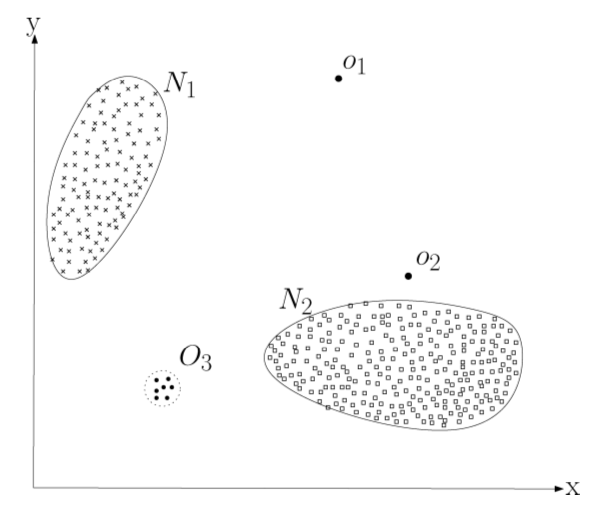
\includegraphics[scale=0.3]{figs/anomaly_example.png}
\caption{\label{fig:anomalyExample}Example of anomalies in a 2D dataset\citep{chandola2009anomaly}.}
\end{figure}



\section{Scikit-learn}
Scikit-learn was chosen as the machine learning library in this project. It is a Python library which is a suitable choice for the project. Alternatively, either Weka or R could be used. Weka is a complete program with GUI, and has an API making it possible to integrate in a Java program. R is a special programming language which is specifically designed for statistical analysis. Scikit-learn depends on \texttt{numpy} and \texttt{scipy} to have the data in correct arrays and to do statistical analysis, and to create graphs is it necessary to use \texttt{matplotlib}. These do not follow in the regular installation of scikit-learn, and will have to be install on its own. 

\subsection{Models}
\glspl{svm} is general terms for models that use supervised learning to analyse and recognize patterns in the data given as a training set. The problem must be binary, which means each point must belong to one of two categories. \gls{ocsvm} is a unsupervised \gls{svm} model, which is  used to solve outlier detection problems. In this project this was needed since the data was not labeled. Elliptical envelope was also used to see the difference between machine learning models. It is a covariance model, and is used to calculate a \gls{mcd}. \gls{mcd} is a function that tries to find a proportion value of the correct observations which is then used to weight the observation to give a better representation \cite{scikit-learn}.
\chapter{Results}
\label{chp:results}



With scikit-learn was a program created in python that reads through the dataset and puts the \gls{dns} calls in to an ndarray, which is a N-dimensional array. This is to easier use to right values for the machine learning model. The program also cleans up the dataset by removing some of the fields, which for this project seemed unnecessary. I created multiple scripts for taking out different sections of the dataset, to see if there would be any difference. The code for the parser program is in \ref{chp:parserprogram}

The main program read through a \texttt{csv} file, the dataset, and put each line as an array in a ndarray. N-dimensional array is a numpy class which is beneficial to use with scikit-learn. Further the ndarray was preprocessed to scale everything to a similar level. This level is set by calculating the mean and standard deviation of the ndarray. 

The different classifiers are initiated with parameters that is changed to see what best fit the data. As the data is unlabeled, it is impossible to know how many of the observations are a part of a \gls{dns} tunnel if there is any. The classifiers must not have any inputs, but it will help making them more precise. In this project the contamination level, which is the level of data which is viewed as incorrect, was first calculated as the percentage of observations which was over average as a base. The value has been change up and down, but kept in the same area. 

To be able to show the solutions and really understand what the machine learning model did, all of the experiments used two dimensions. The dimensions change between $downlink, uplink, duration, downlink/duration$ and $uplink/duration$. The values was not marked with any type, but based on network theory is duration set to the of length of conversation in seconds. The uplink and downlink is  the number of bytes transferred up to the server or downloaded from the server, respectively.

Since it was no known \gls{dns} tunnels in the dataset, it is impossible to use precision, recall or the $F_1$ measure as results. The precision and recall measurements are defined in algorithm \ref{recallPrecision}. The $F_1$ measurement was defined van Rijsbergen \cite{manevitz2002one} as a way of combining precision and recall. The formula is in algorithm \ref{f1}. As seen from the definitions without the knowledge of tunnels in the dataset will there not be a way of measuring the correctness of the machine learning algorithms.

\begin{algorithm}

$$ recall = \frac{Number of items of a category identified}{Number of items in the category in the dataset} $$

$$ precision = \frac{Number of items of a category identified}{Number of items classified to the category} $$

\caption{Recall and precision definitions}
\label{recallPrecision}
\end{algorithm}

\begin{algorithm}
\caption{$F_1$ measure}
\label{f1}
$$ F_1(R,P) = \frac{2RP}{R+P} $$
\end{algorithm}


\begin{figure}[hbp]
\centering
	\begin{subfigure}[b]{0.4\textwidth}
		\centering
		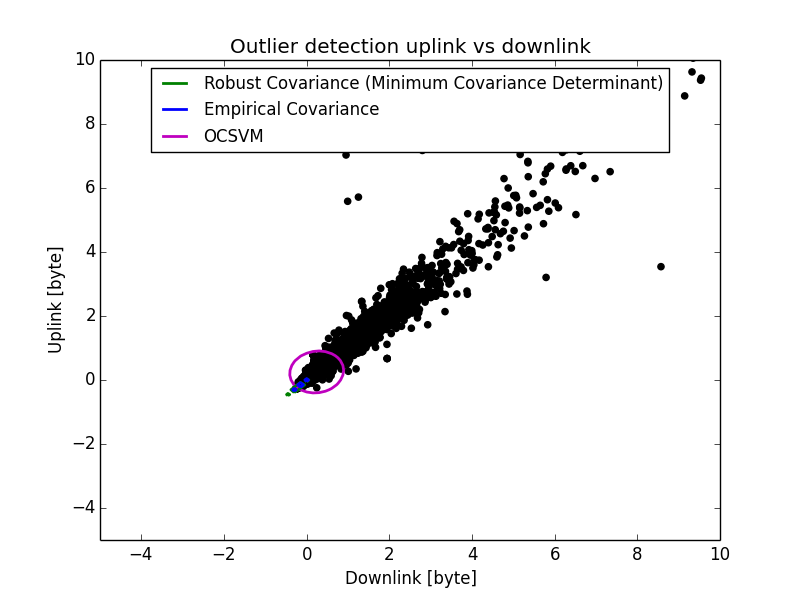
\includegraphics[scale=0.28]{figs/scaleUpVSDown.png}
        \caption{Scaled data}
        \label{fig:scaledUpDown}
	\end{subfigure}
	\begin{subfigure}[b]{0.4\textwidth}
		\centering
		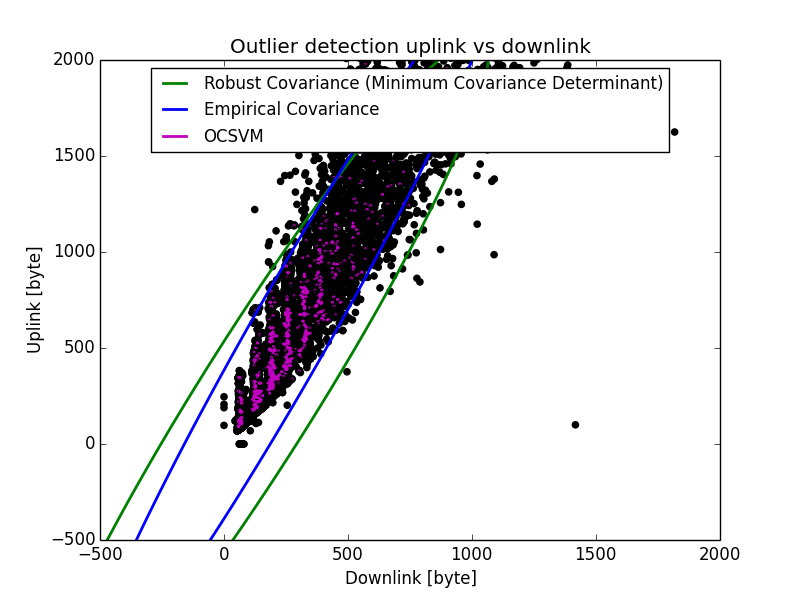
\includegraphics[scale=0.28]{figs/unscaledUpVSDown.png}
		\caption{Unscaled data}
		\label{fig:unscaledUpDown}
	\end{subfigure}
\caption{Difference between scaled and unscaled data}
\label{fig:scaledVSUnscaledUpDown}
\end{figure}


\section{Scaled data vs unscaled data}
As seen in \fref{fig:scaledVSUnscaledUpDown} the scaled and unscaled graphs bears the same characteristics. Most of the observations has almost the same value for uplink and downlink. 
The results were better for \gls{ocsvm} with scaled data, while the covariance calculations worked better with the unscaled. The unscaled data spreads so far out that it is hard to see all the data points, while the scaled data is more compact giving a better overview. The ellipses on the figures is the learned decision of the classifier model. Meaning that inside the ellipses is the area where an observation is considered normal. Since the \gls{ocsvm} is the main focus, scaled data was used for the rest of the experiments.

\section{Different axes}
Next up was looking which values would be best for the axes to represent the data. In \fref{fig:scaledVSUnscaledUpDown} the fields of the dataset used were \texttt{uplink} and \texttt{downlink}. This was the first thoughts of finding irregularities, as mentioned in chapter \ref{chp:dns_detection} is this a volume analysis comparing total volume from a user in one \gls{dns} session. The experiment were then ran with different values to see the difference. In \fref{fig:scaledUpDur} the size of the uploaded data were compared to the time the session were used, this shows that there are a number of users in the same area which the model learn as the normal area, which in scale is around 0. The result were similar when changing uplink with downlink. There are users uploading and downloading lots of data in short time, this lead to the idea of introducing a new field to the dataset. Combining the discoveries from \fref{fig:scaledUpDown} and \fref{fig:scaledUpDur}, by seeing how much data where uploaded or downloaded during a session. This is depicted in \fref{fig:scaledUpDownDivDur}. In this graph it is possible to see that the observation is even more clustered. This seemed like a good representation. 


\begin{figure}
\centering
	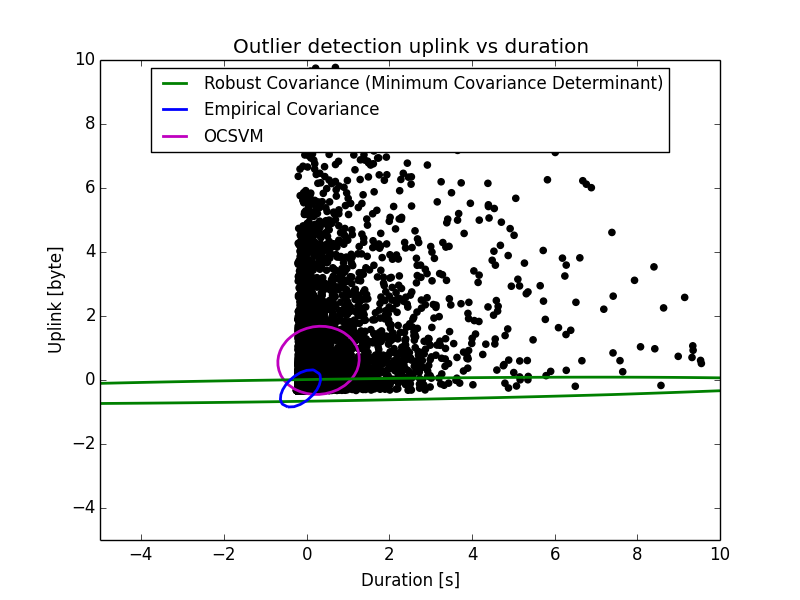
\includegraphics[scale=0.6]{figs/scaleUpVSDur.png}
	\caption{Uplink vs duration of session. }
	\label{fig:scaledUpDur}
\end{figure}


\begin{figure}
	\centering
	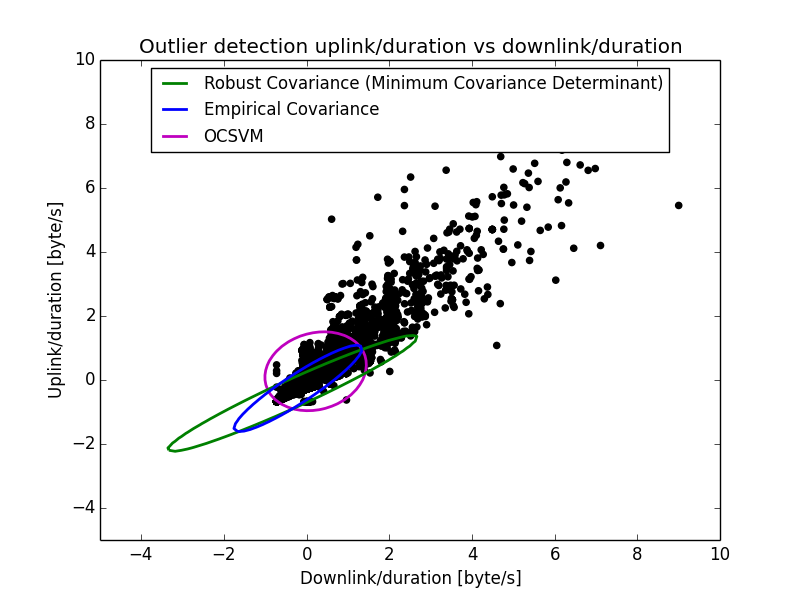
\includegraphics[scale=0.6]{figs/scaleUpDivDurVSDownDivDur.png}
	\caption{Average speed in each direction}
	\label{fig:scaledUpDownDivDur}
\end{figure}

\section{Different parameters}
The fields of the dataset is, as mentioned earlier, not the only variable when finding the best way for a model to fit to the dataset. The machine learning model has parameters that is given when instantiated. For \gls{ocsvm} is it possible to set what kind of kernel it should use and the number of training errors among others. \texttt{Kernel} is the function the model should use. The number of training errors, \texttt{nu} in scikit-learn, is the upper bound fraction of outliers in the training set, and the lower bound of training examples used as support vectors. For this project the kernels used where \texttt{rbf} and \texttt{linear} where rbf is the one used in the graphs so far. 
The nu was first set to $0.15$ which was calculated as the fraction of observations above average, this has been changed to see how it affect the learned decision. In \ref{fig:differentNu} do you see how changing nu is affecting the model. It is clear to see that in this dataset there are a low fraction of observations that does not fit the model. Using the linear kernel the model tries to find a linear line it can draw where all observations on one side is correct observations and on the other side is outliers. This is seen in $ $ $ $ $ $. It was worth a try, but it seems that \texttt{rbf} if the best kernel. 

\begin{figure}
\centering
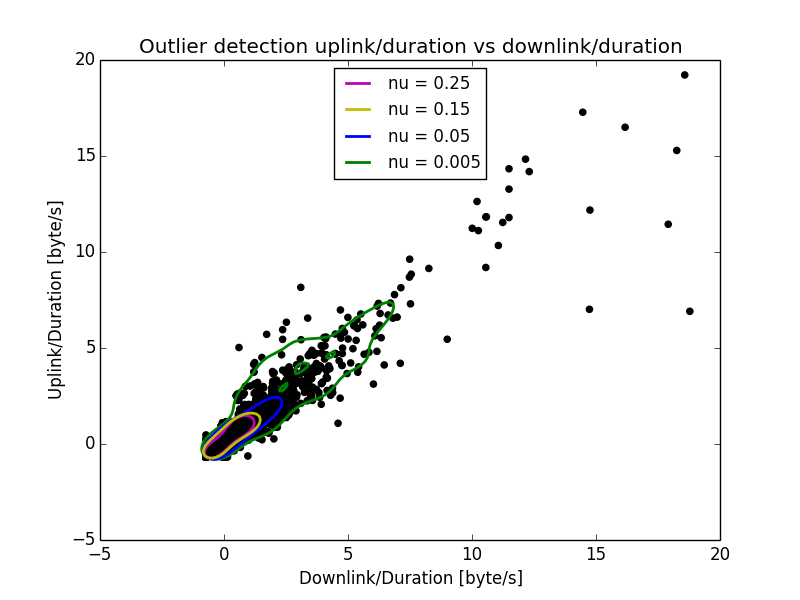
\includegraphics[scale=0.6]{figs/differentNu.png}
\caption{Changing the nu parameter of the \gls{ocsvm}}
\label{fig:differentNu}
\end{figure}



\section{Predicting}
The dataset were also ran through a predicting program where 75 percent of the dataset were used to train the classifier and the last 25 percent were used to test it. Which means that the model tried to give around 5000 observations the correct label. Here the classifier had no problems using more then two features, so the classifier were trained with different features to see how it worked. As seen in table \ref{tab:predicting} is it seen that no matter the features are the predictions quite similar. The one thing to notice is that the more feature used is resulting in a little higher number of outliers, but the change from 33 to 38 out of 5167, is only 0.1 percent change. With $nu = 0.16$ is the percent of outliers around 10 percent, while with $nu = 0.005$ is it only 0.6 percent. \gls{ocsvm} with linear kernel were also tested with prediction but were not nearly as accurate as the rbf kernel. 

\begin{table}
\centering
\begin{tabular}[b]{|c|c|c|c|c|}
\hline
 & \multicolumn{2}{c}{nu = 0.16} & \multicolumn{2}{c}{nu = 0.005} \\ \hline
Features & Outliers & Inliers & Ouliers & Inliers \\ \hline
$Uplink, downlink$ & 438 & 4729 & 29 & 5138 \\ \hline
$Uplink, duration$ & 557 & 4610 & 28 & 5139 \\ \hline
$Downlink, duration$ & 579 & 4588 & 33 & 5134 \\ \hline
$Uplink, downlink, duration$ & 568 & 4599 & 38 & 5129 \\ \hline
$\frac{Uplink}{duration}, \frac{downlink}{duration }$ & 469 & 4698 & 26 & 5141 \\ \hline
$Uplink, downlink, duration, \frac{Uplink}{duration}, \frac{downlink}{duration }$ & 613 & 4554 & 36 & 5131 \\ \hline
\end{tabular}
\caption{\label{tab:predicting} Number of observations classified as outliers and inliers with different features and nu value} 
\end{table} 
\chapter{Conclusion}
\label{chp:conclusion}

\section{Conclusion}
With the results the experiments have yielded, seen in chapter \ref{chp:results}, does it looks like machine learning is a good way of detecting \gls{dns} tunnels. The classifier model \gls{ocsvm} with the default kernel \texttt{rbf}, does create a good decision function which the graphs shows. The table \ref{tab:predicting} shows that the predicting function also gives good results. Even though it is not possible to say if it is completely correct. The dataset is unlabeled and might not contain a \gls{dns} tunnel, but the results gives indication of sessions and users which should be inspected. The Elliptical envelope model has the disadvantage that it has to create a ellipse as the decision function which seems to make inaccurate either making the decision function cover a very large or too small area. As seen in \ref{fig:scaledUpDownDivDur} mot the Robust Covariance and the Empirical Covariance cover smaller area of observations and larger area of blank space than the \gls{ocsvm}. The linear kernel of \gls{ocsvm} finds a linear function in which observation on one side is the inliers and the other side is the outliers. This showed some results with some of the features, but was worse than the rbf kernel overall.


\section{Future work}
With the findings in this project could it be interesting doing experiments where with data know to contain a \gls{dns} tunnel, either continue with unlabeled learning or label the data and to supervised learning. This could also be tested against one another. Also creating a program which could take in a real time data stream and give out suspicious connection based on this model or the best model from the previous experiment mentioned, making it a complete program for tunnel detection. There are also more to data to look at to make a complete detection program. The dataset contained also had information about other services the user did. Combining more features might be of help, e.g. look if an user makes a \texttt{http} request after the \gls{dns} session or what kind of data plan the user has. 

\renewcommand*{\bibname}{References}
\bibliographystyle{alpha}
\bibliography{main}

%% Uncomment the following if you have any appendix
\appendix
\addtocontents{toc}{%
  \protect\vspace{1em}% 
  \protect\noindent \bfseries \appendixtocname\protect\par
  \protect\vspace{-.5em}%
 }
 \renewcommand{\chaptername}{\appendixname}
%% include below possible appendices (chapters)
\chapter{Parser program}
\label{chp:parserprogram}

\begin{Verbatim}
import csv

def allDnsCalls(csvIn):
	#opens the outputfile
	with open('allDnsCalls.csv', 'wb') as writefile:
		spamwriter = csv.writer(writefile, delimiter=',', quotechar='|')
		for row in csvIn:
			#Remove values though as unecessary for the experiment
			row.pop(-1)
			row.pop(-2)
			row.pop(-2)
			#9000 where the representing value for a DNS call
			if row[0] == '9000':
				row.pop(0)
				#calculate uplink/duration and downlink/duration
				if float(row[-1]) == 0:
					bpsUp = row[1]
					bpsDown = row[2]
				else:
					bpsUp+ = float(row[1])/float(row[-1])
					bpsDown = float(row[2])/float(row[-1])
				
				row.append(bpsUp)
				row.append(bpsDown)
				spamwriter.writerow(row)

#Opens the dataset file
with open('ggsnSample-4Kristofer-hashIMSI.csv','rb') as csvfile:
	spamreader = csv.reader(csvfile, delimiter=',', quotechar='|')
	allDnsCalls(spamreader)
\end{Verbatim}

\end{document} 
